% Auto-included at the end of Section 6. Every number below is read from
% figures/data/*.csv (derived by figures/scripts/extract_flywheel.py).
\subsection{Where training stands}\label{sec:method-status}
We report the live training loop as it is, not as we hope it will be.
\Cref{fig:fw-validation} shows every candidate the adapter proposed over
695 consecutive rounds (rounds 775--1469). Only 4 were admitted; the best
validation utility, 1.1378, has not been exceeded since. \Cref{fig:fw-trainval}
shows the reason we treat this as a plateau rather than a pause: on every
logged round, training utility sits 0.282--0.290 above validation utility, a
generalization gap that further adapter steps have not closed. The frozen
encoder's checksum matched on every round; only the adapter trains.
\Cref{fig:fw-telemetry} gives the loop's operating envelope.

\begin{figure}[t]
  \centering
  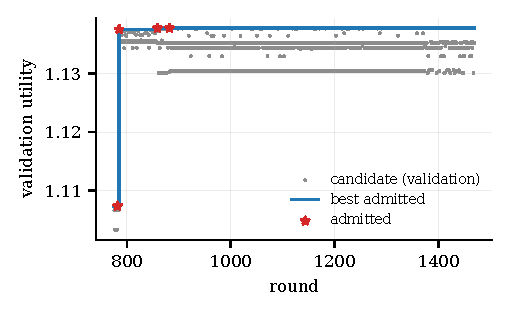
\includegraphics[width=\linewidth]{figures/fig_fw_validation.pdf}
  \caption{\textbf{Validation utility has plateaued.} Grey: each round's
  candidate adapter on the validation families. Blue: best admitted model.
  Stars: the four admitted candidates (rounds 775--1469).}
  \label{fig:fw-validation}
\end{figure}

\begin{figure}[t]
  \centering
  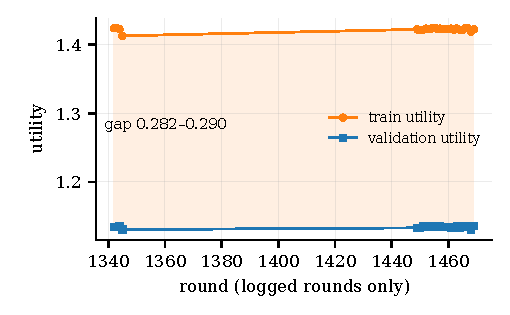
\includegraphics[width=\linewidth]{figures/fig_fw_train_val.pdf}
  \caption{\textbf{Train and validation utility, with the gap shown.} Only
  rounds whose full summaries are retained are plotted (25 rounds between
  1342 and 1469); the line joins non-consecutive rounds across the gap.}
  \label{fig:fw-trainval}
\end{figure}

\begin{figure*}[t]
  \centering
  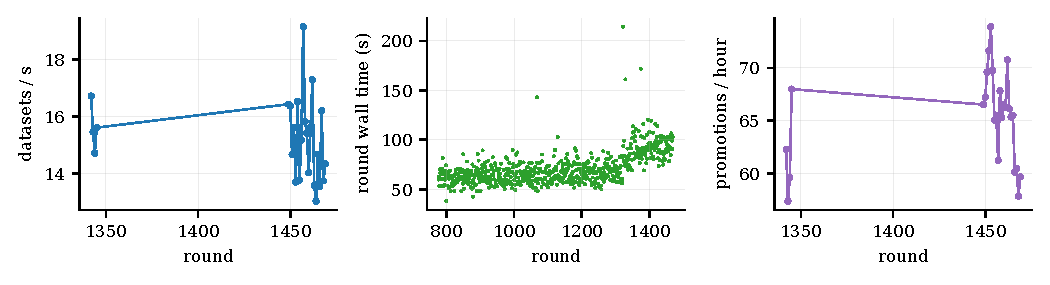
\includegraphics[width=\linewidth]{figures/fig_fw_telemetry.pdf}
  \caption{\textbf{Loop telemetry.} Left: datasets evaluated per second.
  Middle: wall time between consecutive rounds. Right: programs promoted into
  the pools per hour. The run directory occupied 290\,MB at the snapshot.}
  \label{fig:fw-telemetry}
\end{figure*}
